\documentclass{article}
\usepackage{kotex}
\usepackage{kotex-logo}
\usepackage{graphicx}  % 사진, 그림 삽입
\usepackage[cmyk, dvipsnames, svgnames]{xcolor}  % 색
\definecolor{SunOrange}{cmyk}{0, .47, .78, 0}  % 색상 정의{c, m, y, b(k)}
\usepackage[framemethod=tikz]{mdframed}  % 상자
\usepackage{tabularx}  % 표 만들기에 필요한 패키지들
\usepackage{booktabs}
\usepackage{array}
\usepackage{makeidx}  % 색인
\makeindex 

\title{근본없는 \LaTeX 설명서}
\author{Dokenzy}
\date{2026.06.25.THU}

\begin{document}
\maketitle        % 제목
\tableofcontents  % 목차
% 그림의 차례: listoffigures, 표의 차례: listoftables

\section{첫걸음}
\begin{itemize}   % 라벨링(기호)
\item 좋아하는 연예인
\item[-] 좋아하는 텍스트 편집기
\item 우리 동네에 있는 카페 
\end{itemize}

\begin{enumerate} % 라벨링(숫자)
\item 좋아하는 연예인
\item 좋아하는 텍스트 편집기
\item 우리 동네에 있는 카페
\end{enumerate}

우쭈쭈\index{우쭈쭈} % 인덱싱(색인)

\section{기본 명령과 환경} % 상호참조
\label{hello}
이번 장은 \pageref{hello}쪽에 있는 
\ref{hello}절입니다.\footnote{각주는 여기에 나타납니다.}  % 각주
폰트 크기를 조절하고 싶다면 중괄호로 감싸서 {\tiny 특정 부분만 조절할 수 있도록} 하자
만약 폰트 크기 조절을 문단 전체에 적용하고 싶다면 명령 대신 환경을 이용하자.

\begin{footnotesize}
문단 전체 글씨가 각주 크기로 나타납니다.
문단 전체 글씨가 각주 크기로 나타납니다.
문단 전체 글씨가 각주 크기로 나타납니다.
문단 전체 글씨가 각주 크기로 나타납니다. 
\end{footnotesize}

\section{필수 패키지}
\begin{itemize}
\item graphicx
: 이미지를 넣기 위해 쓰이는 패키지. 이미지 파일이름은 확장자를 빼고 이름만 넣도록 한다.
label 명령을 활용할 때는 반드시 caption 명령 뒤에 입력해야 상호참조 가능하다.

\begin{figure}[!hbp]
    \centering
    \caption{wallpaper}
    \label{fig: wallpaper}
    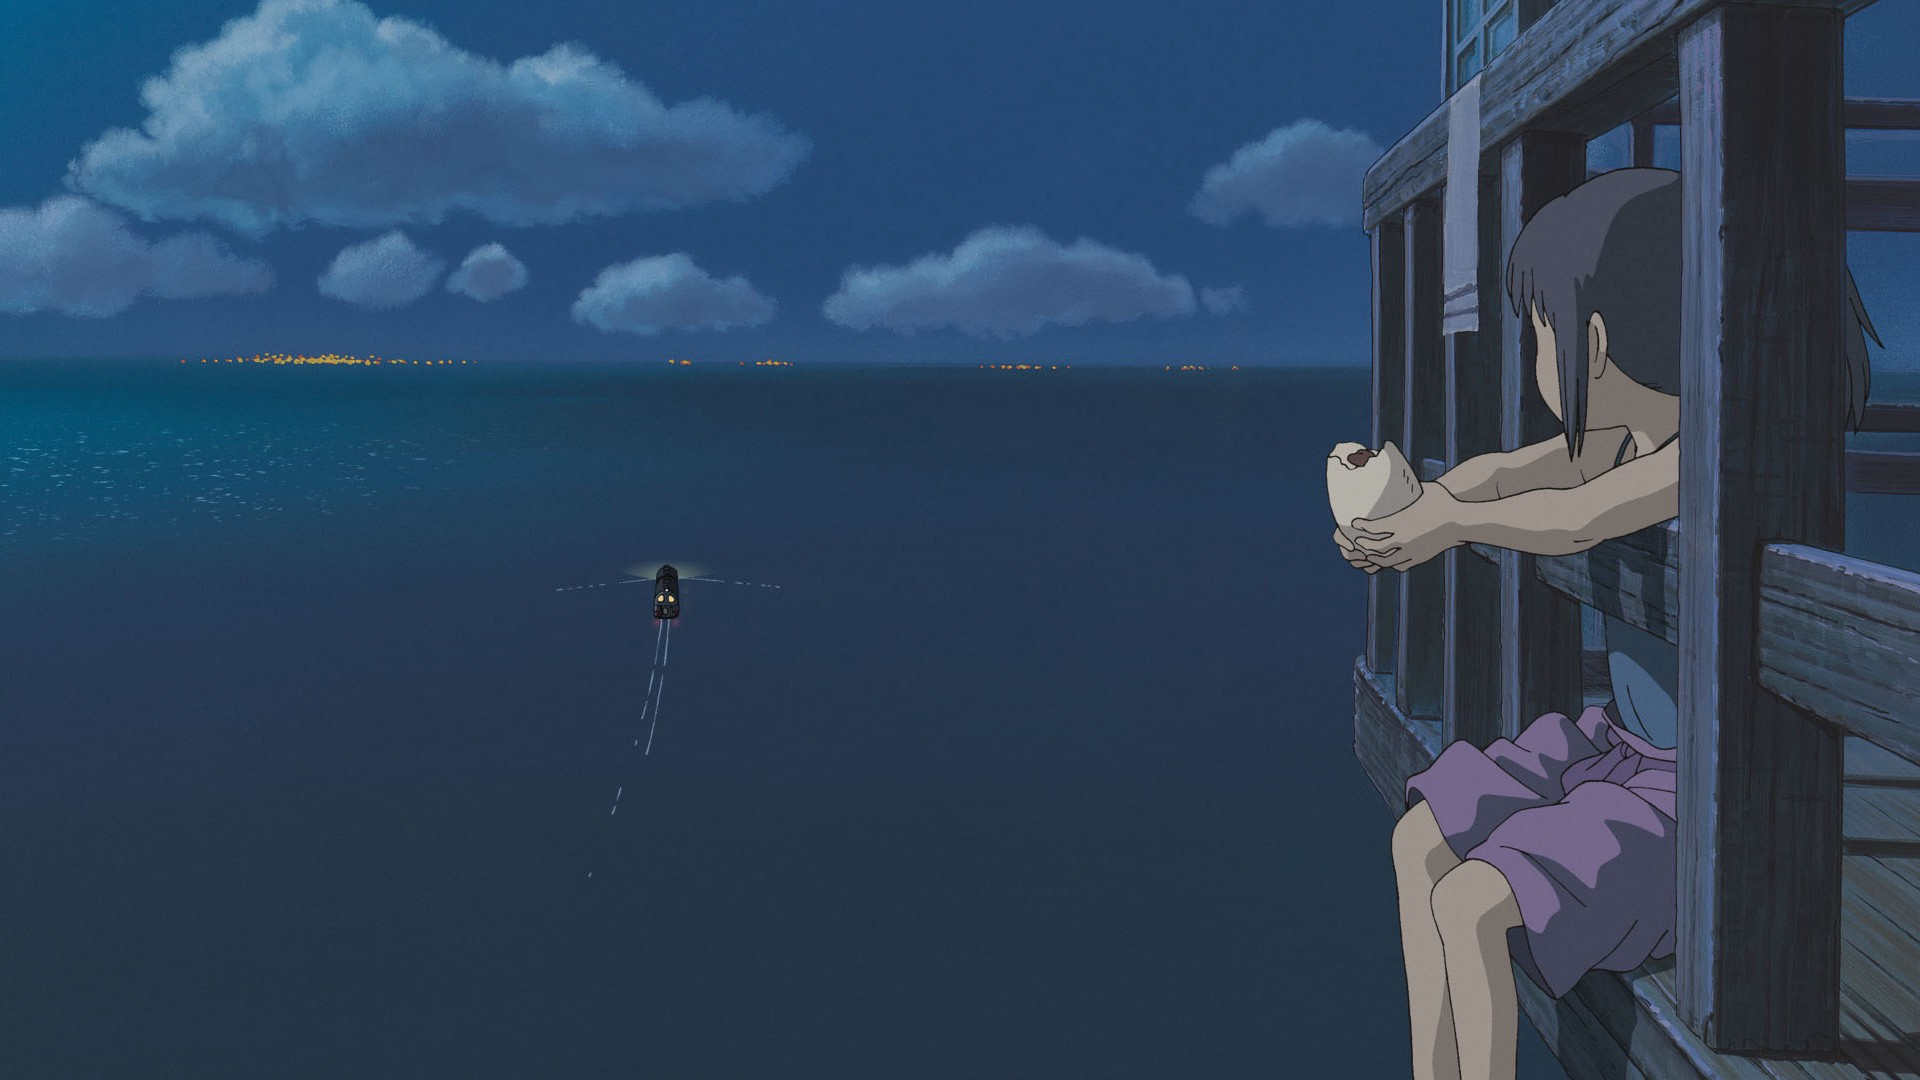
\includegraphics[
        width=0.5\textwidth,
        height=5cm,
        angle=0]{wallpaper}
\end{figure}

\item xcolor
: 색을 다루는 패키지. 나는 \textcolor{HotPink}{핫핑크}가 좋아.
\textcolor{SunOrange}{햇빛오렌지색}

\item mdframed
: 박스를 꾸밀 때 필요한 패키지
    \begin{mdframed}[
    linecolor = Green!80, 
    roundcorner = 10pt, 
    backgroundcolor = Green!10,
    innertopmargin=\topskip,
    frametitleaboveskip=2pt,
    frametitlefont=\bfseries\itshape,
    frametitlerule=true, 
    frametitlerulewidth=1pt,
    frametitlebackgroundcolor=Olive!20,
    frametitlealignment=\center,
    leftmargin=1cm, 
    rightmargin=1cm, 
    frametitle={\normalfont\bfseries\Large%
    \color{DodgerBlue}푸리에 급수의 부분합}]
디리클레는 푸리에 급수의 부분합을 아래와 같이 나타냈습니다.
\[ 
S_n(x) = \frac{1}{\pi}\int_{\pi}^{\pi}f(t)\frac{sin(n+1/2)(t-x)}{sin(t-x)/2}dt
\] 
    \end{mdframed}

\item hyperref
: 문서 작성 중 링크를 만들 때 사용하는 패키지.
\item tabularx
: 표를 만들 때 사용하는 패키지. 
\begin{tabularx}{\linewidth}{cXXX}
\toprule
$x$ (도) & $\sin x$ & $\cos x$ & $\tan x$ \\
\midrule
\sffamily 0 & 0 & 1 & 0 \\
1 & 0.0174524 & 0.99984769 & 0.01745506 \\
2 & 0.03489949 & 0.99939082 & 0.03492076 \\
3 & 0.05233595 & 0.99862953 & 0.05240777 \\
\bottomrule
\end{tabularx}
\end{itemize}

\section{폰트}
참고 자료가 오래된 관계로 활용할 수 있는 폰트 관련 내용 無
\\ 폰트에 대한 학습은 추후 따로 진행하는 것으로 하겠음. 

\section{Minimal Working Example}
대부분의 오류는 다음과 같은 경우에 발생한다. 
\begin{itemize}
\item 오타
\item 괄호의 짝이 맞지 않을 때
\item $\backslash begin\{\}, \backslash end\{\}$ 짝이 맞지 않을 때
\item 없는 명령이나 환경을 사용했을 때
\item 옵션을 잘못 사용했을 때
\end{itemize}

오류메시지를 잘 읽어보면 어느 부분에서 오류가 발생했는지 알 수 잇지만, 오류 원인을 알아내는 것이 매번 쉬운 일은 아님.
이때, Minimal Working Example(MWE)를 만들면 오류의 원인을 비교적 쉽게 찾아낼 수 있다. 
\begin{footnotesize}
MWE 만드는 파트도 잠시 유보하도록 하자. 설명이 미비하게 나와있다. 
\end{footnotesize}

\section{\koTeX{}과 oblivoir로 한국어 문서 조판하기}
\subsection{\koTeX}
\koTeX{}이 제공하는 기능은 다음과 같다. 자세한 내용은 \koTeX 설명서 참조
\begin{itemize}
    \item 우리말 이름(장, 절, 차례 등)
    \item 방점
    \item 한글식 카운터
    \item 자동조사
    \item 미세조정(자간, 어간, 행간 등)
    \item 찾아보기, 참고문헌 등
    \item 옛한글
    \item 한글문서 서식
    \item 세로쓰기
\end{itemize}
\subsection{oblivoir 클래스}
memoir 클래스에 \koTeX을 내장한 클래스. 자세한 설명은 oblivoir의 설명서 `texdoc oblivoir' 참고

\section{좀 더 \LaTeX스럽게}
\subsection{간단한 사용자 정의 명령}
예를 들어 비야네 스트롭스트룹(Bjarne Stroustrup)에 대해 글을 쓴다고 하자. 
이 사람의 이름이 자연스레 여러 번 쓰일 것이므로, 사용자 정의 명령을 통해 입력을 간단히 할 수 있다.
$\backslash newcommand\{\}$ 명령어를 통해 새로운 명령을 정의할 수 있으며, 
이미 정의한 것을 다시 정의해야 할 일이 생기면 $\backslash renewcommand\{\}$을 활용하자. 
둘의 사용법은 같다. 
\newcommand{\bjarne}{Bjarne Stroustrup}
\bjarne
\subsection{옵션이 있는 사용자 정의 명령}
\newcommand{\sunnytext}[2][SunOrange]{\textcolor{#1}{#2}}
기본색은 \sunnytext{햇빛오렌지색}이지만, 
다른색상도 사용할 수 있다. \sunnytext[Goldenrod]{Goldenrod}색
\printindex        % 색인출력 

\end{document}